	
\section{Codificación de Voz}

Las redes de datos transfieren la información de modo digital y en VoIP la información que se maneja son señales de audio, principalmente señales de voz. Estas señales son analógicas por naturaleza, así que se requiere de un mecanismo que digitalice las señales analógicas, es decir, convierta las señales de voz en una secuencia de números discreta, para luego poder ser enviadas por la red y haga el proceso inverso al llegar a destino. 
Sí la solución VoIP implementada es completamente digital, éste proceso ocurre directamente en el teléfono (teléfonos digitales, celulares, micrófonos de computadores); en cambio, sí el sistema incluye secciones combinadas con telefonía tradicional, el proceso de digitalización ocurre en las intersecciones de los sistemas, bien sea en las pasarelas (gateways) del sistema o en conectores ATA (Analog Thelephone Adapter) como se muestra en las siguientes figuras
[FIGURA \ref{fig:pasarela}]  [FIGURA \ref{fig:ata}].

	\begin{figure}[h]
		
		%nombre de la imagen, sin extencion. "width=\textwidth" ancho igual al texto
		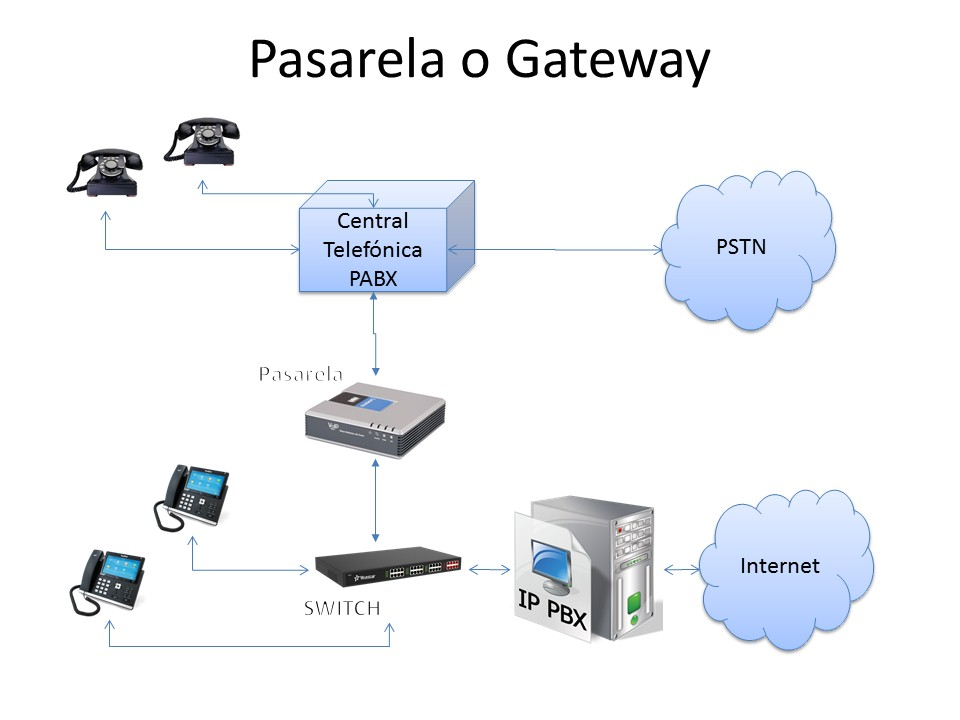
\includegraphics[scale=0.5]{pasarela}
		
		%titulo de la imagen, salen debajo de la imagen y en el indice de imagenes.
		\caption{VoIP combinada con telefonía tradicional a través de una pasarela}
		
		%centrado, por si las moscas
		\centering
		
		%para referencias
		\label{fig:pasarela}
	\end{figure}

Los primeros trabajos sobre digitalización de audio fueron realizados por el Ingeniero Alec Reeves poco antes de la segunda guerra mundial, quien desarrolló un sistema de audio digital con fines militares, sin embargo, la tecnología de comunicaciones de la época todavía no estaba lista para dicho avance. Alec Reeves patento un total de 82\footnote{http://www.quiantium.plus.com/ahr/patents.htm}  inventos entre los que se destaca la idea de Modulacion por impulsos codificados (PCM, Pulse Coded Modulation). Alrededor de los 60s fue que se popularizó la tecnología de PCM pero para entonces ya no eran reclamables los derechos de la patente.

	
		\begin{figure}[h]
			
			%nombre de la imagen, sin extencion. "width=\textwidth" ancho igual al texto
			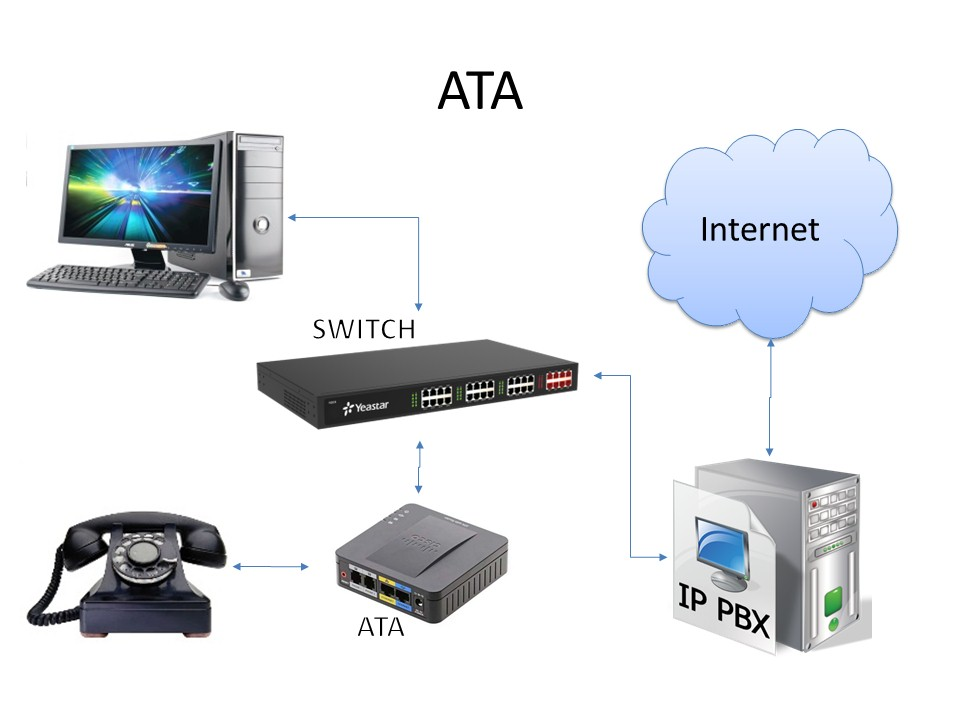
\includegraphics[width=\textwidth]{ata}
			
			%titulo de la imagen, salen debajo de la imagen y en el indice de imagenes.
			\caption{VoIP usando teléfonos analógicos y ATAs}
			
			%centrado, por si las moscas
			\centering
			
			%para referencias
			\label{fig:ata}
		\end{figure}
		
		
Inicialmente la digitalización de voz se basó en codificar la forma de onda de la señal analógica mediante un proceso de muestreo, cuantificación y codificación de la señal, el proceso de PCM. Luego, con el objetivo de reducir la tasa de bits requerida para transmitir la señal, se introdujeron las técnicas predictivas y comenzaron a codificar solo la diferencia entre los valores de las muestras reales y la predicción de la señal en base a la extrapolación de las muestras anteriores.

\subsection{Proceso de digitalización}

Las señales analógicas pasan por un proceso de conversión de tres etapas antes de convertirse en señales digitales. Aunque las especificaciones técnicas de cada etapa dependen directamente del códec utilizado, el proceso general es similar y se ilustra en la siguiente [FIGURA \ref{fig:procesoDigitalizacion}]

	\begin{figure}[h]
	
		%nombre de la imagen, sin extencion. "width=\textwidth" ancho igual al texto
		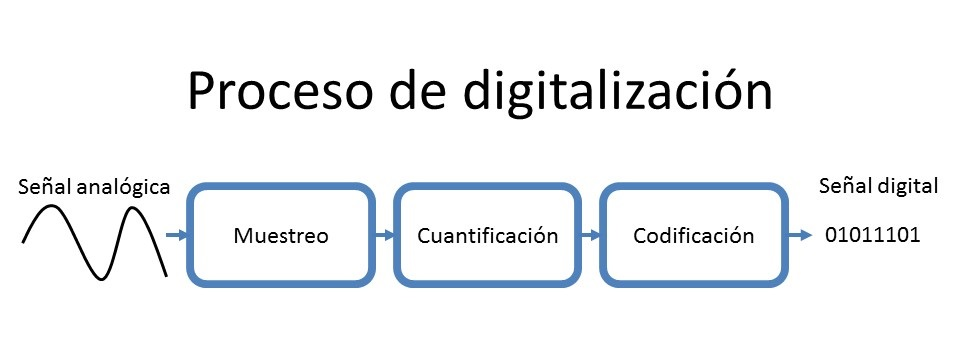
\includegraphics[width=\textwidth]{procesoDigitalizacion}
		
		%titulo de la imagen, salen debajo de la imagen y en el indice de imagenes.
		\caption{Proceso general de digitalización.}
		
		%centrado, por si las moscas
		\centering
		
		%para referencias
		\label{fig:procesoDigitalizacion}
	\end{figure}

\subsubsection{Muestreo}
El proceso de muestreo consiste en tomar muestras de la señal de audio en intervalos regulares de tiempo. Para que en este proceso de digitalización no exista pérdida de información, se debe tomar muestras de la señal a una velocidad (frecuencia de muestreo) que sea, como mínimo, el doble \cite{nyquist} de la frecuencia más alta presente en la señal que se convierte. Cada códec tiene una frecuencia de muestreo definida en su estándar, y depende del tipo de banda (angosta, amplia, super-amplia o completa) que utilice el códec. En la siguiente [Figura \ref{fig:muestreo}] se ilustra el resultado de esta etapa.

	\begin{figure}[h]
		%nombre de la imagen, sin extencion. "width=\textwidth" ancho igual al texto
		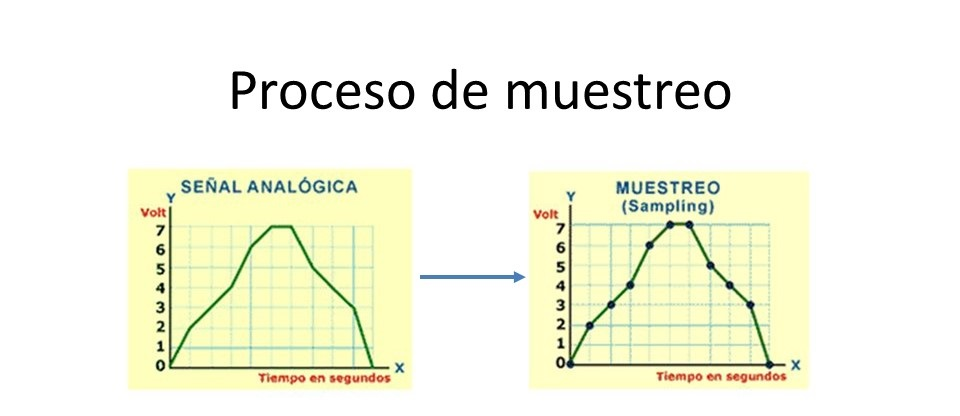
\includegraphics[width=\textwidth]{muestreo}
		
		%titulo de la imagen, salen debajo de la imagen y en el indice de imagenes.
		\caption{Resultado del muestreo de una señal analógica.}
		
		%centrado, por si las moscas
		\centering
		
		%para referencias
		\label{fig:muestreo}
	\end{figure}

\subsubsection{Cuantificación}
El proceso de cuantificación convierte las muestras obtenidas en la etapa anterior en valores discretos, los cuales se pueden “medir” según una escala determinada por cada códec. Cuantos más valores discretos se utilicen, menor será la distorsión o ruido introducido por el proceso de digitalización, pero se necesitará mayor cantidad de bits para poder procesar o transmitir la información. En la siguiente [Figura \ref{fig:cuantificacion}] se ilustra el resultado de esta etapa.

	\begin{figure}[h]
		%nombre de la imagen, sin extencion. "width=\textwidth" ancho igual al texto
		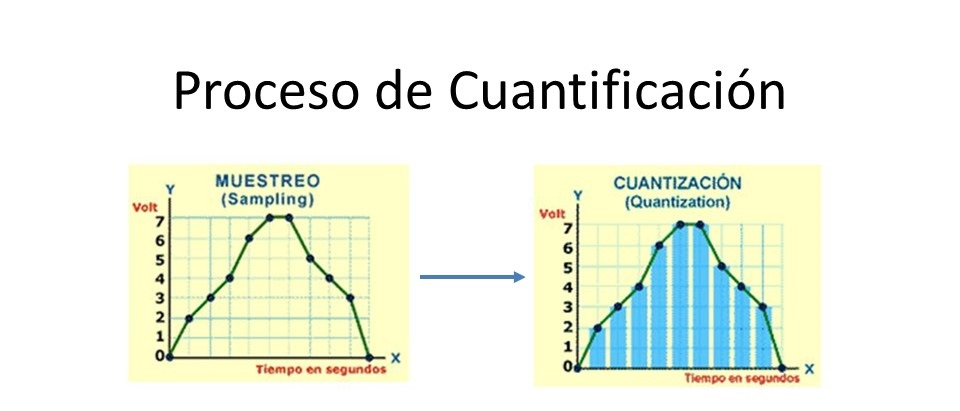
\includegraphics[width=\textwidth]{cuantificacion}
		
		%titulo de la imagen, salen debajo de la imagen y en el indice de imagenes.
		\caption{Resultado de la cuantificación de una señal muestreada.}
		
		%centrado, por si las moscas
		\centering
		
		%para referencias
		\label{fig:cuantificacion}
	\end{figure}

\subsubsection{Codificación}
Una vez que las muestras tienen un valor discreto asignado, estos deben ser traducidos a un formato que sea manejable digitalmente como es el caso de valores binarios. En la siguiente [Figura \ref{fig:codificacion}] se ilustra el resultado de esta etapa. 

	\begin{figure}[h]
		%nombre de la imagen, sin extencion. "width=\textwidth" ancho igual al texto
		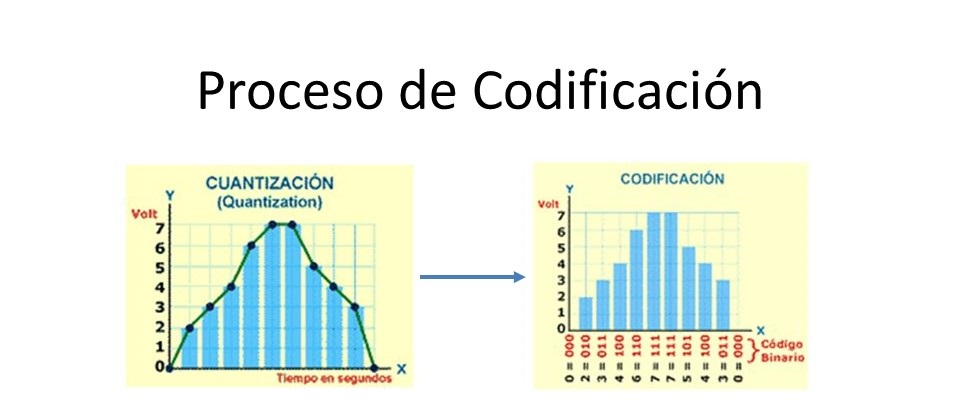
\includegraphics[width=\textwidth]{codificacion}
		
		%titulo de la imagen, salen debajo de la imagen y en el indice de imagenes.
		\caption{Resultado de la codificación de muestras cuantificadas.}
		
		%centrado, por si las moscas
		\centering
		
		%para referencias
		\label{fig:codificacion}
	\end{figure}

\subsection{Códec}

Los códec son algoritmos o dispositivos que realizan la codificación y decodificación de la señal de audio, con usados a menudo en videoconferencias y emisiones de medios de comunicación. La mayoría de los códec provoca pérdidas de información ya que están diseñados para minimizar el tamaño de los datos digitales. Existen códec sin pérdida (lossless) que mantienen la calidad más precisa del sonido, pero generan datos digitales muy grandes que en VoIP no son necesarios.

		\begin{table}[h]
			
			%nombre de la imagen, sin extencion. "width=\textwidth" ancho igual al texto
			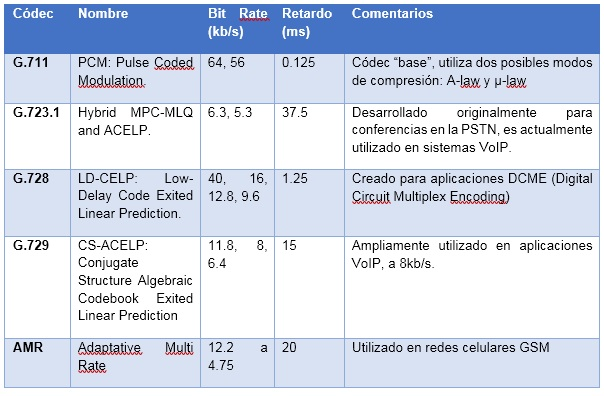
\includegraphics[width=\textwidth]{../tables/codecsnarrowband}
			
			%titulo de la imagen, salen debajo de la imagen y en el indice de imagenes.
			\caption{Códec de banda angosta (Narrowband).}
			
			%centrado, por si las moscas
			\centering
			
			%para referencias
			\label{tab:narrow}
		\end{table}


Existe gran variedad de códecs en el mercado actual y su clasificación puede depender de varios aspectos como la técnica que usan para codificar, el ancho de banda que se muestra o incluso la tasa de bits resultante. En las siguientes tablas se puede apreciar las principales diferencias entre los códec más comunes. En la primera [\ref{tab:narrow}] se pueden apreciar los principales códec de banda angosta, diseñados para digitalizar audio en frecuencias entre 300Hz y 3,4kHz. En la segunda [\ref{tab:wide}] se comparan los códec de banda ancha que reproducen señales entre 50Hz y 7kHz. En la tercera [\ref{tab:full}] se encuentran los códec de banda super amplia (frecuencias de 50Hz a 14kHz) y banda completa (frecuencias de 50 Hz a 20 kHz).

	\begin{table}[h]
	
		%nombre de la imagen, sin extencion. "width=\textwidth" ancho igual al texto
		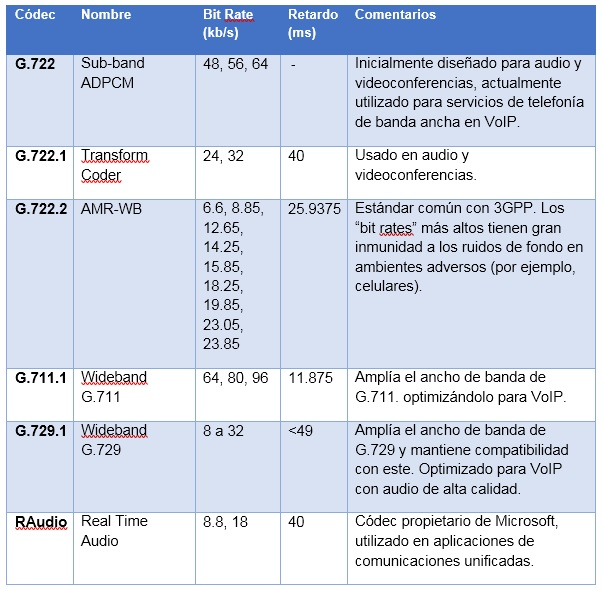
\includegraphics[width=\textwidth]{../tables/codecswideband}
		
		%titulo de la imagen, salen debajo de la imagen y en el indice de imagenes.
		\caption{Códec de banda ancha (Wideband).}
		
		%centrado, por si las moscas
		\centering
		
		%para referencias
		\label{tab:wide}
	\end{table}

	\begin{table}[h]
	
		%nombre de la imagen, sin extencion. "width=\textwidth" ancho igual al texto
		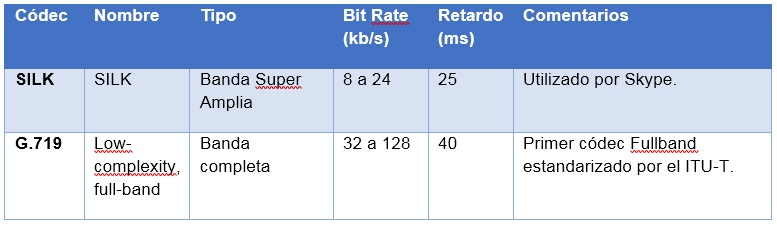
\includegraphics[width=\textwidth]{../tables/codecfullband}
		
		%titulo de la imagen, salen debajo de la imagen y en el indice de imagenes.
		\caption{Códec de banda superancha (Superwideband ) y Completa (Fullband).}
		
		%centrado, por si las moscas
		\centering
		
		%para referencias
		\label{tab:full}
	\end{table}
	

\subsubsection{G.711}

El códec básico y más antiguo en telefonía es el estandarizado en la recomendación G.711 de la ITU-T, está enfocado en reproducir la “forma de onda” de la señal y su cuantificación, de tipo “no lineal” puede hacerse de acuerdo a dos leyes, “ley A” o “ley u” \cite{g711}. 

Como G.711 es un códec de banda angosta, su frecuencia de muestreo es de 8kHz, es decir, se toma una muestra cada 125 microsegundos. Si bien esta frecuencia es adecuada para reproducir la voz humana, con cierto grado de perdida, no es adecuada para audio de alta calidad con frecuencias máximas de 20kHz.

Se ha demostrado que el oído humano es más sensible a ruidos en señales de baja amplitud que a los mismos ruidos en señales de mayor amplitud. Por lo tanto, al tener una cuantificación de tipo “no lineal” se acepta tener distorsiones grandes en las partes de mayor amplitud de la señal mientras que en las partes de baja amplitud de la señal las distorsiones sean más pequeñas. 

Tanto la cuantificación como la codificación de las señales, con éste códec, dependen directamente de la ley implementada. Estas “leyes de compresión” estandarizan en 256 niveles no lineales la cuantificación y codificación de la voz en telefonía basadas en fórmulas matemáticas bien definidas, sin embargo la implementación real utiliza 13 segmentos de recta que se aproximan a la formula teórica de la “Ley A” y 15 segmentos aproximados a la formula teórica de la “Ley u“. Para información más detallada de cada ley se sugiere revisar la recomendación G.711 \cite{g711}.

\subsubsection{G.711.1}

El códec G.711.1 es una extensión a banda amplia del códec original G.711. En su modo “banda amplia” codifica señales de hasta 7kHz y está optimizado para VoIP. Una característica interesante de este códec es su compatibilidad hacia atrás. Por lo que toma muestras a 16kHz en su modo amplio y a 8kHz en su modo de compatibilidad. Las tramas son de 5ms por lo que la perdida de paquetes no afecta en gran medida a la reconstrucción de la señal. En la siguiente [FIGURA \ref{fig:g7111}]\footnote{Extraído de www.adaptivedigital.com/products/vocoders/g.711.1.pdf} se puede apreciar los modos de operación de este códec.

	\begin{figure}[h]
		%nombre de la imagen, sin extencion. "width=\textwidth" ancho igual al texto
		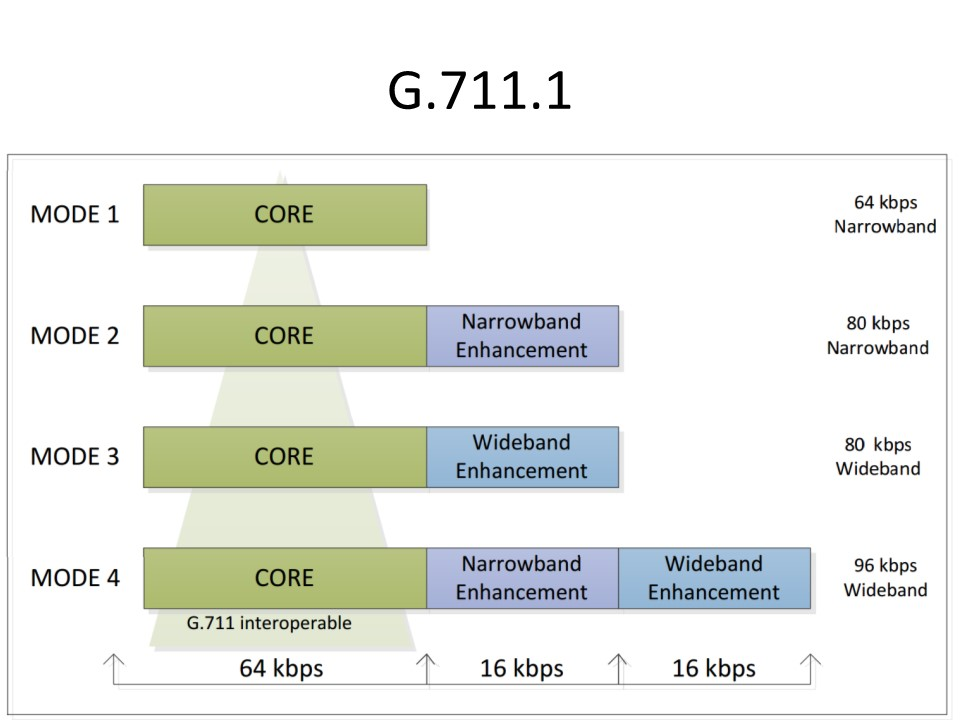
\includegraphics[width=\textwidth]{g7111}
		
		%titulo de la imagen, salen debajo de la imagen y en el indice de imagenes.
		\caption{Modos de operación del G.711.1}
		
		%centrado, por si las moscas
		\centering
		
		%para referencias
		\label{fig:g7111}
	\end{figure}

\subsubsection{G.722}
El códec G.722 separa la señal de audio en dos bandas y las codifica por separado usando la técnica ADPCM (Adaptative Differential Pulse Code Modulation). Puede operar  a veocidades de 64, 56 y 48 kbits/s. En los últimos dos casos es posible enviar un canal auxiliar de información de 8 o 16 kbit/s respectivamente, completando así una velocidad constante de 64kbit/s.

\subsubsection{G.723.1}
El códec G.723.1 codifica las señales de voz a 6,4 o 5,3 kbit/s usando ventanas de 30ms. Para la velocidad de 6,4 kbit/s utiliza el algoritmo MP-MLQ (Multi-Pulse Maximun Likelihood Quantization), generando 24 bytes de datos por cada ventana de 30ms. Para la velocidad de 5,3 kbit/s se utiliza ACELP, generando 20 bytes por cada ventana de 30ms (Algebraic Code Excited Linear Prediction).

El anexo A de la recomendación G.723.1 ayuda a reducir el ancho de banda utilizado al no transmitir muestras durante los periodos de silencio.

\subsubsection{G.729}
El códec G.729 codifica las señales a 8 kbit/s utilizando CS-ACELP (Conjugate-Structure Algebraic-Code-Exited Liner Prediction). Utiliza ventanas de 10ms generando 10 bytes de datos por ventana.

El Anexo A del códec define una variante que reduce su complejidad y es compatible hacia atrás con el códec original.

El Anexo B de la recomendación G.729 provee detección de actividad de voz y silencios, ayudando a disminuir el ancho de banda utilizado al no enviar muestras durante los periodos de silencio.

\subsubsection{G.729.1}
El códec G.729.1 amplia el espectro de frecuencias del códec G.729. Fue diseñado para facilitar la interoperabilidad entre las redes de banda angosta (300 a 3400 Hz) y las redes de banda ancha (50 a 7000 Hz). 
La señal codificada tiene una tasa de bits de 8 a 12 kbit/s para señales de banda angosta y de 14 a 32 kbit/s para señales de banda ancha. Las tramas de salida consisten en 12 capas, como se muestra en la [FIGURA \ref{fig:g7291}]. 

\begin{figure}[h]
	%nombre de la imagen, sin extencion. "width=\textwidth" ancho igual al texto
	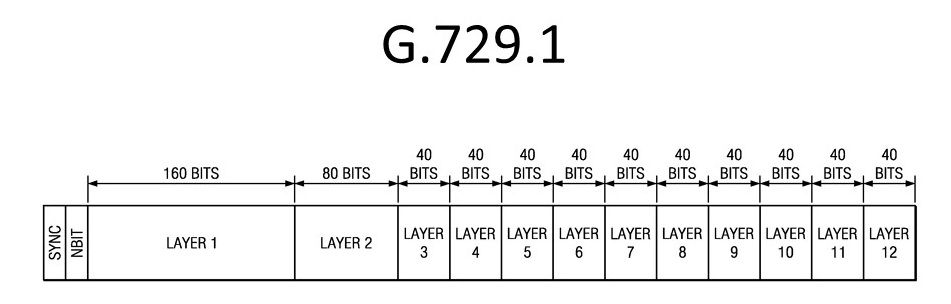
\includegraphics[width=\textwidth]{g7291}
	
	%titulo de la imagen, salen debajo de la imagen y en el indice de imagenes.
	\caption{Capas del códec G.729.1}
	
	%centrado, por si las moscas
	\centering
	
	%para referencias
	\label{fig:g7291}
\end{figure}

La capa 1 corresponde a 8 kbit/s y utiliza la codificación CELP, siendo compatible con G.729. La capa ocupa 4kbit/s y corresponde a mejoras en las frecuencias de la banda angosta. Las siguientes capas ocupan 2kbit/s cada una y corresponden a mejoras en las frecuencias de banda ancha.

Las tramas son de 20ms y puede ser truncada a la salida del codificador, en el decodificador, o cualquier otro punto de la red, si fuera necesario reducir el ancho de banda.

\subsubsection{RTAudio}
El códec RTAudio fue desarrollado por Microsoft y ha sido usado comercial y cooperativamente. Utiliza 8,8 kbit/s de ancho de banda y técnicas LPC (Linear Prediction Coefficients). RTAudio utiliza técnicas VBR (Variable Bit Rate), lo que significa que no todas las ventanas o muestras se codifican con la misma cantidad de bytes.

\subsubsection{SILK}
El códec SILK fue utilizado por SKYPE. Utiliza un ancho de banda variable, entre  6 y 40 kbit/s. Éste códec puede trabajar en banda angosta y banda ancha, con tramas de 20 ms y un retardo de 25 ms.
 
SILK fue reemplazado por el códec OPUS, el cual fue aceptado con el RFC 6716--REFERENCIA NECESARIA.  

